\scanpage{10}

forment un syst. projectif \inserted{strict} d'algèbres sur $A$.
$\mathcal C_i(G)_f$ est équivalente \unsure{canoniqut} à la catégorie des $\mathcal U_i$-modules \inserted{de t.f.}. Et les foncteurs \unsure{transition} entre les $\mathcal C_i(G)$ sont isomorphes aux \deleted{\unsure{aux}} foncteurs \uline{restriction des scalaires}.

\uline{Corollaire} Sous les conditions précédentes, tt module \inserted{de t.f.} $E$ d'une représentation de $G$ est quotient d'un module \inserted{\uline{projectif}} de t.f. où $G$ opère.
\margin{\figure{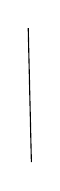
\begin{tikzpicture}[x=1cm,y=1cm]\draw (0,0)--(-.04,1.7);\end{tikzpicture}}}

\uline{Prop.} Soit $G$ gr. affine plat sur $A$ anneau de Dedekind, d'algèbre $B$ satisfaisant aux conditions du lemme 1. (NB. si $G$ est de t.f. cela signifie que pour tte composante irréd. de $G$, \uline{toutes} ses fibres sont non vides).

Soit \deleted{$A'$ une $A$-algèbre} $S'$ un schéma sur $S$, tel que sur $S$, tt module quasi-coh de t.f. \deleted{admette \unsure{un}} \inserted{soit isomorphe} à un quotient d'un module loc. libre de t.f. \deleted{Alors} (p.ex. $S$ est \unsure{noeth.} \unsure{imm. quasi-proj.|immers. quasi-proj.}, ou $S$ noeth. régulier). Alors tt

\mspage{9}
